\documentclass[a4paper,12pt]{article}
\usepackage[a4paper,top=1.3cm,bottom=2cm,left=1.5cm,right=1.5cm,marginparwidth=0.75cm]{geometry}
\usepackage{cmap}
\usepackage{mathtext}
\usepackage[T2A]{fontenc}
\usepackage[utf8]{inputenc}
\usepackage[english,russian]{babel}
\usepackage{siunitx}

\usepackage{graphicx}

\usepackage{wrapfig}
\usepackage{tabularx}

\usepackage{hyperref}
\usepackage[rgb]{xcolor}
\hypersetup{
colorlinks=true,urlcolor=blue
}
\usepackage{amsmath,amsfonts,amssymb,amsthm,mathtools}
\usepackage{icomma}
\mathtoolsset{showonlyrefs=false}
\usepackage{euscript}
\usepackage{mathrsfs}
\DeclareMathOperator{\sgn}{\mathop{sgn}}
\newcommand*{\hm}[1]{#1\nobreak\discretionary{}
{\hbox{$\mathsurround=0pt #1$}}{}}

%%% Заголовок
\author{Макаров Лев Евгеньевич}
\title{Лабораторная работа №1.4.1

Изучение экспериментальных погрешностей на примере физического маятника
}
\date{\today}


\begin{document}

\begin{titlepage}
	\begin{center}
		{\large МОСКОВСКИЙ ФИЗИКО-ТЕХНИЧЕСКИЙ ИНСТИТУТ (НАЦИОНАЛЬНЫЙ ИССЛЕДОВАТЕЛЬСКИЙ УНИВЕРСИТЕТ)}
	\end{center}
	\begin{center}
		{\large Физтех-школа фотоники, электроники и молекулярной физики}
	\end{center}
	
	
	\vspace{4.5cm}
	{\huge
		\begin{center}
			{\bf Отчёт о выполнении лабораторной работы 1.2.4}\\
			Определение главных моментов инерции твердых тел с помощью крутильных колебаний
		\end{center}
	}
	\vspace{2cm}
	\begin{flushright}
		{\LARGE Автор:\\ Макаров Лев Евгеньевич \\
			\vspace{0.2cm}
			Б04-306}
	\end{flushright}
	\vspace{8cm}
	\begin{center}
		Долгопрудный 2023
	\end{center}
\end{titlepage}


\section{Введение}

\textbf{Цель работы:} 
\begin{enumerate}
	\item измерить периоды крутильных колебаний рамки при различных положениях закрепленного в ней тела
	\item проверить теоретическую зависимость между периодами крутильных колебаний тела относительно различных осей
        \item определить моменты инерции относительно нескольких осей для каждого тела, по ним найти главные моменты инерции тела и посторить эллипсоид инерции
\end{enumerate}

\textbf{В работе используются:} 
\begin{itemize}
    \item установка для получения крутильных колебаний
    \item набор исследуемых твердых тел
    \item секундомер
    \item штангенциркуль
    \item электронные весы ВЛТЭ-5100
\end{itemize}
\medskip


\section{Теоретические сведения}
\subsection{Общие сведения}

Инерционные свойства твердого тела при вращении определяется
пространственным распределением массы. Оно характеризуется величиной, называемой тензором инерции. Тензор инерции твердога тела может быть предствален симметричной матрицей, которая полностью определяется заданием шести эллементов:

\begin{equation*}
\hat{I} = \left(
\begin{array}{ccc}
I_{xx} & I_{xy} & I_{xz} \\
I_{yx} & I_{yy} & I_{yz} \\
I_{zx} & I_{zy} & I_{zz} \\
\end{array}
\right)
\end{equation*}

Элемент $I_{ij}, \text{ где } i,j \in \{ x, y, z \}$ внаходится по формуле:

\begin{equation}\label{xx}
    I_{xx} = \int \left(y^2 + z^2 \right) dm, I_{yy} = \int \left(x^2 + z^2 \right) dm, I_{zz} = \int \left(x^2 + y^2 \right) dm
\end{equation}
\begin{equation}
    I_{xy} = I_{yx} = - \int xy dm, I_{xz} = I_{zx} = - \int xz dm, I_{yz} = I_{zy} = - \int yz dm
\end{equation}

Момент инерции относительно произвольной оси, проходящей через начало координат, может быть вычислен по формуле:
 
\begin{equation}
    I = \sum_{i,j=x}^{z} \left( I_{ij} s_{i} s_{j} \right)
\end{equation}

Матрица тензора инерции может быть приведена к диагональному виду, диагональные элементы $I_{x}$, $I_{y}$, $I_{z}$ которой называются главными моментами инерции тела. Геометрическим представлением тензора инерции является эллипсоид, уравнение которого в главных осях имеет вид:

\begin{equation}
    I_{x} x^2 + I_{y} y^2 + I_{y} y^2 = 1
\end{equation}

Данный эллипсоид называется эллипсоидом инерции. Координатные оси $Ox$, $Oy$, $Oz$ совпадают с главными осями тела. если начало координат $O$ совпадает с центром масс, то эллипсоид называется центральным. Зная эллипсоид инерции можно найти момент инерции тела относительно оси, проходящий через центр эллипсоида. Для этого влдоль выбранной оси необходимо провести радиус-вектор $\vec{r}$ до пересечения с поверхностью эллипсоида. Момент инерции относительно этой оси определяется так:

\begin{equation}
    I = \frac{1}{r^2}
\end{equation}

В данной работе используется устройство для получения крутильных колебаний, изображенное на \textit{рис.  \ref{ustan}}. Рамка 1 жестко соединена с проволокой 2, закрепленной вертикально в специальных зажимах 3, позволяющих сообщить начальное закручивание для возбуждения крутильных колебаний вокруг вертикальной оси. В рамке с помощью планки 4, гаек 5 и винта 6 закрепляется твердое тело 7. На теле имеются специальные выемки, позволяющие его закрепить так, чтобы ось вращения проходила в теле под различными углами через цеитр масс.

\begin{figure}[h!]
        \centering
	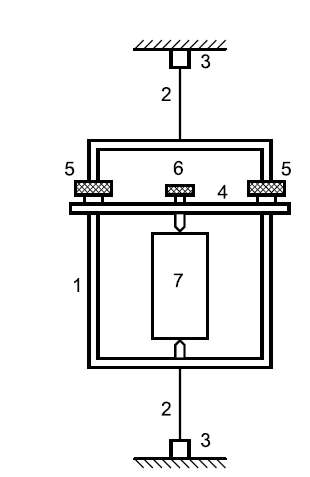
\includegraphics[width=0.3\textwidth]{ustan.png}
	\caption{\textit{Схема установки}}
	\label{ustan}
\end{figure}

Крутильные колебания рамки с телом описываются уравнением:

\begin{equation}
    \left( I + I_{p} \right) \frac{d^2 \varphi}{dt^2} = - f \varphi
\end{equation}

Здесь $I$ и $I_{p}$ -- моменты инерции тела и рамки относительно оси вращения, $\varphi$ -- угол поворота рамки, меняющийся со верменем $t$, $f$ -- модуль кручения проволоки. Период крутильных
 колебаний рамки с телом определяется формулой:
 
\begin{equation}
    T = 2\pi\sqrt{\frac{I+I_{p}}{f}}
\end{equation}

На \textit{рис.  \ref{cube}} показано, как проходят оси вращения в параллелепипеде.
 Оси АА', BВ' и СС' являются главными. Моменты инерции относительно
этих осией обозначим соотственно $J_{x}, J_{y}, J_{z}$.\\

\begin{figure}[h!]
        \centering
	\includegraphics[width=0.3\textwidth]{cube.png}
	\caption{\textit{Оси вращения прямоугольного параллелепипеда}}
	\label{cube}
\end{figure}

Момент инерции $I_{D}$ при вращении относительно диагонали DD' выражается
 через главные моменты с помощью формулы:
 
\begin{equation}\label{main-d}
    I_{d}=I_{x}\frac{a^2}{d^2}+I_{y}\frac{b^2}{d^2}+I_{z}\frac{c^2}{d^2}
\end{equation}

Используя связь момента инерции с периодом крутильных колебаний
получаем соотношение между периодами колебаний относительно осей DD', ЕE',
ММ' и PР' с периодами крутильных колебаний относительно главных осей.

\begin{equation}\label{verify1}
    (a^2+b^2+c^2)T^2_{D}=a^2 T^2_{x}+b^2 T^2_{y}+c^2 T^2_{z},
\end{equation}

\begin{equation}\label{verify2}
    (b^2+c^2)T^2_{E}=b^2 T^2_{y}+c^2 T^2_{z},
\end{equation}

\begin{equation}\label{verify3}
    (a^2+c^2)T^2_{P}=a^2 T^2_{x}+c^2 T^2_{z},
\end{equation}

\begin{equation}\label{verify4}
    (a^2+b^2)T^2_{M}=a^2 T^2_{x}+b^2 T^2_{y},
\end{equation}

Эти соотношения также необходимо проверить экспериментально.

\subsection{Момент инерции различных тел}

Момент игерции параллелепипеда со сторонами $a$, $b$, $c$ можно вычислить следующим образом относительно оси z по формуле \eqref{xx}:

\begin{multline*}
    I_{z} = \int \left(x^2 + y^2 \right) dm = \rho \int_{-\frac{c}{2}}^{\frac{c}{2}} \int_{-\frac{b}{2}}^{\frac{b}{2}} \int_{-\frac{a}{2}}^{\frac{a}{2}} (x^2 + y^2 ) dx \text{ } dy \text{ } dz = \\
    = \rho c \int_{-\frac{b}{2}}^{\frac{b}{2}} \left( \int_{-\frac{a}{2}}^{\frac{a}{2}} (x^2 + y^2 ) dx \right) dy = \rho c \int_{-\frac{b}{2}}^{\frac{b}{2}} \left( \frac{a^3}{12} + y^2 a \right) dy =
\end{multline*}

\begin{equation}\label{cilinder-z}
    = \frac{\rho abc}{12} (a^2 + b^2) = \frac{m}{12} (a^2 + b^2)
\end{equation}

Относительно двух других осей момент инерции выводится аналогично:

\begin{equation}\label{cilinder-xy}
    I_{x} = \frac{m}{12} (b^2 + c^2), I_{y} = \frac{m}{12} (a^2 + c^2)
\end{equation}

Момент инерции $I_\text{AC'}$ относительно оси, проходящей через главную диагональ вычисляется по формуле \eqref{main-d}:

\begin{equation}\label{cilinder-AC}
    I_\text{AC'} = \frac{m}{12d^2} \left(a^2 (b^2 + c^2) + b^2 (a^2 + c^2) + c^2 (a^2 + b^2) \right) = \frac{m}{6d^2} \left( a^2 b^2 + a^2 c^2 + b^2 c^2 \right)
\end{equation}

Моменты инерции $I_\text{MM'}$, $I_\text{EE'}$, $I_\text{PP'}$ относительно оси, проходящей через MM', EE', PP' соответственно вычисляются по формулам:

\begin{equation}\label{cilinder-MM}
    I_\text{MM'} = I_{x} \frac{a^2}{a^2 + b^2} + I_{y} \frac{b^2}{a^2 + b^2}
\end{equation}

\begin{equation}\label{cilinder-EE}
    I_\text{EE'} = I_{x} \frac{a^2}{a^2 + c^2} + I_{z} \frac{c^2}{a^2 + c^2}
\end{equation}

\begin{equation}\label{cilinder-PP}
    I_\text{PP'} = I_{y} \frac{b^2}{b^2 + c^2} + I_{z} \frac{c^2}{b^2 + c^2}
\end{equation}

Для куба моменты инерции относительно данных осей вычисляются аналогично, только у куба: $a = b = c$.


Для цилиндра момент инерции относительно оси HH', проходящей параллельно его высоте через центр его масс, вычисляется по формуле: 

\begin{equation}\label{actual-cil-h}
    I_\text{выс} = \int r^2 dm = \rho \int r^2 dV = \rho \int_0^R r^2 \text{ } 2 \pi r h \text{ } dr = \rho \int_0^R 2 \pi r^3 h \text{ } dr = 2 \pi h \rho \int_0^R r^3 \text{ } dr = 2 \pi h \rho \frac{R^4}{4} = \frac{mR^2}{2}
\end{equation}

Для вычисления момента инерции $I_\text{диам}$ цилиндра относительно оси DD', проходящей через его центр масс параллельно диаметру, представим цилиндр как совокупность тонких дисков толщиной $dh$, массой $dm = \frac{m}{H} dh$. Момент инерции тонкого диска относительно оси DD' $dI$ вычисляется в соответствии с теоремой Гюйгенса-Штейнера:

\begin{equation}
    dI = \frac{dmR^2}{4} + dmh
\end{equation}

Здесь $h$ - расстояние от центра масс цилиндра до центра тонкого диска. Момент инерции $I_\text{диам}$ вычисляется так:

\begin{equation}\label{actual-cil-d}
    I_\text{диам} = \int^{\frac{H}{2}}_{-\frac{H}{2}} \left( \frac{dmR^2}{4} + dmh \right) = \int^{\frac{H}{2}}_{-\frac{H}{2}} h^2 \frac{m}{H} dh + \frac{mR^2}{4} = \frac{mH^2}{12} + \frac{mR^2}{4}
\end{equation}

\section{Оборудование и экспериментальные погрешности}

\textbf{Секундомер:} $\sigma_s = \pm 0,06$ с \\ 
\textbf{Электронные весы ВЛТЭ-5100:} $\sigma_m = \pm 0,1$ г \\
\textbf{Штангенциркуль:} $\sigma_\text{шт} = \pm 0,005$ см \\

\section{Результаты измерений и обработка данных}
\subsection{Проверка установки}

Перед началом выполнения работы необходимо убедиться в том, что установка работает корректно:
\begin{enumerate}
    \item Проволока должна быть хорошо натянута
    \item Рамка должна быть жёстко закреплена
    \item Устройство для возбуждения крутильных колебаний
    \item Отсутствие колебаний в векртикальной плоскости
\end{enumerate}

\subsection{Использование установки}

Научимся закреплять тела в рамке. На телах имеются специальные углубления, в которые должны входить винты, имеющиеся на рамке. Для закрепления тела в рамке (\textit{рис. \ref{ustan}}) нужно, отвернув гайки 5, под- нять вверх подвижную планку 4 на рамке, вставить тело в рамку, попав углублением, имеющимся на теле, на выступ нижней стороны рамки. Опуская планку, необходимо выступающим из плавки на 5-7 мм вин- том 6 попасть в отверстие на теле. Закрепив планку гайками 5, немного подожмите тело винтом 6. Если в дальнейшем обнаружится, что тело поворачивается в рамке, надо его еще поджать винтом 6. После того, как мы научились пользоваться установкой, можно приступать к выполнению работы.

\subsection{Выбор амплитуды колебаний}

Амплитуда колебаний должна быть выбрана так, чтобы после 15 колебаний она уменьшалась менее, чем в два раза. Такая амплитуда достигается при двух последовательных разгонах с использованием устройства для возбуждения крутильных колебаний (устройство включено от момента прохождения маятником начального положения до момента достижения максимальной амплитуды) и составляет приблизительно $45^\circ$. Данное значение амплитуды будет использоваться во время всех измерений.

\subsection{Измерение периодов колебаний}

Для пустой рамки измерим время 15 колебаний три раза:

\begin{table}[!ht]
    \centering
    \begin{tabular}{|l|l|l|}
    \hline
        № изм & T, с & t, с \\ \hline
        1 & 67,62  & 4,51 \\ \hline
        2 & 66,84  & 4,46 \\ \hline
        3 & 67,26  & 4,48 \\ \hline
    \end{tabular}\caption{\textit{Измерение периода колебаний для рамки}}
\end{table}

Систематическая погрешность вычисления периода одного колебания $t$ равна: $\sigma_t^\text{сист} = \frac{\sigma_s}{15} = 0,04 \text{ с}$.

Среднее значение периода $ \overline{t} = \frac{\sum t_i}{N} = 4,48 \text{ с}$.\\

Случайная погрешность измерения $ \sigma_{\overline{t}} = \sqrt{\frac{1}{N  (N-1)}\sum(t_i-\overline{t})^2} \approx 0,02 \text{ с}$. \\

Полная погрешность измерения периода колебаний рамки может быть вычислена так:

\begin{equation}
    \sigma^{\text{полн}}_{\overline{t}} = \sqrt{\left( \sigma_{\overline{t}} \right)^2 + \left( \sigma_t^\text{сист} \right) ^ 2} \approx 0,04 \text{ с}
\end{equation}

\begin{equation}
    t_{\text{р}} = ( 4,48 \pm 0,04 ) \text{ с}
\end{equation}

Проведём аналогичные измерения для параллепипеда, только относительно 7 различных осей, изображённых на \textit{рис. \ref{cube}}. В таблицу \ref{almost_cube} сразу запишем значение $t = \frac{T}{15}$:

\begin{table}[!ht]
    \centering
    \begin{tabular}{|l|l|l|l|l|l|l|l|}
    \hline
        № изм & $t_X$, с & $t_Y$, с & $t_Z$, с & $t_\text{MM'}$, с & $t_\text{EE'}$, с & $t_\text{PP'}$, с & $t_\text{AC'}$, с \\ \hline
        1 & 7,00 & 6,53 & 5,65 & 6,66 & 5,81 & 5,97 & 6,03  \\ \hline
        2 & 7,03 & 6,53 & 5,64 & 6,24 & 5,80 & 5,97 & 6,06  \\ \hline
        3 & 7,02 & 6,60 & 5,65 & 6,66 & 5,82 & 5,98 & 6,06  \\ \hline
        ср & 7,01 & 6,55 & 5,65 & 6,52 & 5,81 & 5,97 & 6,05  \\ \hline
    \end{tabular}\caption{\textit{Измерение периода колебаний параллепипеда для различных осей}}\label{almost_cube}
\end{table}

Так как все измерения отличаются от среднего менее, чем на систематическую погрешность измерения, то случайной погрешностью измерения можно пренебречь.

Проведём аналогичные измерения для куба и двух цилиндров и запишем в таблицы (блином обозначается цилиндр с меньшей высотой):

\begin{table}[!ht]
    \centering
    \begin{tabular}{|l|l|l|l|}
    \hline
        N изм  & $t_X$, с & $t_\text{MM'}$, с & $t_\text{AC'}$, с \\ \hline
        1  & 5,35 & 5,35 & 5,35  \\ \hline
        2  & 5,37 & 5,35 & 5,39  \\ \hline
        3  & 5,34 & 5,37 & 5,37  \\ \hline
        ср & 5,35 & 5,36 & 5,37  \\ \hline
    \end{tabular}\caption{\textit{Измерение периода колебаний куба для различных осей}}\label{cube-t}
\end{table}

\begin{table}[!ht]
    \centering
    \begin{tabular}{|l|l|l|}
    \hline
        N изм  & $t_\text{выс}$, с & $t_\text{диам}$, с \\ \hline
        1  & 6,03 & 5,34  \\ \hline
        2  & 6,04 & 5,36  \\ \hline
        3  & 6,00 & 5,34  \\ \hline
        ср & 6,02 & 5,34  \\ \hline
    \end{tabular}\caption{\textit{Измерение периода колебаний блина для различных осей}}\label{cilinder1}
\end{table}

\begin{table}[!ht]
    \centering
    \begin{tabular}{|l|l|l|}
    \hline
        N изм  & $t_\text{выс}$, с & $t_\text{диам}$, с \\ \hline
        1  & 5,63 & 5,31  \\ \hline
        2  & 5,57 & 5,29  \\ \hline
        3  & 5,67 & 5,29  \\ \hline
        ср & 5,62 & 5,30  \\ \hline
    \end{tabular}\caption{\textit{Измерение периода колебаний цилиндра для различных осей}}\label{cilinder1}
\end{table}

Измерения периода крутильных колебаний для пустой рамки запишем в табоицу \ref{ramka}.

\begin{table}[!ht]
    \centering
    \begin{tabular}{|l|l|}
    \hline
        N изм  & $t_\text{р}$, с \\ \hline
        1  & 4,51  \\ \hline
        2  & 4,46 \\ \hline
        3  & 4,48  \\ \hline
        ср & 4,48  \\ \hline
    \end{tabular}\caption{\textit{Измерение периода колебаний для пустой рамки}}\label{ramka}
\end{table}

Как видно, для всех измерений значения отличаются от среднего не более, чем на систематическую погрешность, поэтому случайной погрешностью измерения можно пренебречь. Погрешность для всех измерений составит $\sigma_t = 0,04 \text{ с}$.

\subsection{Измерение параметров тел и вычисление моментов инерции}

С помощью штангенциркуля и электронных весов измерим соответственно геометрические параматры тел и их массы и запишем в таблицы:

\begin{table}[!ht]
    \centering
    \begin{tabular}{|l|l|}
    \hline
        \textbf{Цилиндр} & ~ \\ \hline
        Характеристика & Значение \\ \hline
        масса, г & 2263,8 \\ \hline
        высота, см & 4,90 \\ \hline
        диаметр, см & 8,80 \\ \hline
    \end{tabular}\caption{\textit{Измерение параметров цилиндра}}
\end{table}

\begin{table}[!ht]
    \centering
    \begin{tabular}{|l|l|}
    \hline
        \textbf{Блин} & ~ \\ \hline
        Характеристика & Значение \\ \hline
        масса, г & 1569,5 \\ \hline
        высота, см & 1,19 \\ \hline
        диаметр, см & 12,45 \\ \hline
    \end{tabular}\caption{\textit{Измерение параметров блина}}
\end{table}

\begin{table}[!ht]
    \centering
    \begin{tabular}{|l|l|}
    \hline
        \textbf{Куб} & ~ \\ \hline
        Характеристика & Значение \\ \hline
        масса, г & 1569,5 \\ \hline
        сторона, см & 9,26 \\ \hline
    \end{tabular}\caption{\textit{Измерение параметров куба}}
\end{table}

\begin{table}[!ht]
    \centering
    \begin{tabular}{|l|l|}
    \hline
        \textbf{Параллелепипед} & ~ \\ \hline
        Характеристика & Значение \\ \hline
        масса, г & 1569,5 \\ \hline
        a, см & 5,04 \\ \hline
        b, см & 10,01 \\ \hline
        c, см & 15,00 \\ \hline
    \end{tabular}\caption{\textit{Измерение параметров параллелепипеда}}
\end{table}

Теперь рассчитаем главные моменты инерции для тел. Для параллелепипеда воспользуемся формулами \eqref{cilinder-z}, \eqref{cilinder-xy}, \eqref{cilinder-AC}, \eqref{cilinder-EE}, \eqref{cilinder-MM}, \eqref{cilinder-PP} и результат запишем в таблицу \ref{paral-i}.

\begin{table}[!ht]
    \centering
    \begin{tabular}{|l|l|l|l|l|l|l|l|}
    \hline
        Ось & Ox & Oy & Oz & MM' & EE' & PP' & AC' \\ \hline
        I, $\text{г } \cdot \text{м}^2$ & 5,644 & 4,346 & 2,180 & 4,609 & 2,531 & 2,847 & 3,050 \\ \hline
        $\sigma_{I}$, $\text{г } \cdot \text{м}^2$ & 0,003 & 0,003 & 0,002 & 0,003 & 0,002 & 0,002 & 0,004 \\ \hline
        $\varepsilon_{I}$, $\%$ & 0,06 & 0,06 & 0,09 & 0,05 & 0,08 & 0,06 & 0,12 \\ \hline
    \end{tabular}\caption{\textit{Моменты инерции для различных осей параллелепипеда}}\label{paral-i}
\end{table}

Погрешности вычисляются по следующим формулам и тоже занесены в таблицу \ref{paral-i}:

\begin{equation}
    \sigma_{I_{x}} = \sqrt{
    \left( \frac{dI_{x}}{dm} \right)^2 \sigma_{m}^2 + 
    \left( \frac{dI_{x}}{db} \right)^2 \sigma_{b}^2 + 
    \left( \frac{dI_{x}}{dc} \right)^2 \sigma_{c}^2
    } \approx 0,003 \text{ г } \cdot \text{м}^2
\end{equation}

\begin{equation}
    \sigma_{I_{y}} = \sqrt{
    \left( \frac{dI_{y}}{dm} \right)^2 \sigma_{m}^2 + 
    \left( \frac{dI_{y}}{da} \right)^2 \sigma_{a}^2 + 
    \left( \frac{dI_{y}}{dc} \right)^2 \sigma_{c}^2
    } \approx 0,003 \text{ г } \cdot \text{м}^2
\end{equation}

\begin{equation}
    \sigma_{I_{z}} = \sqrt{
    \left( \frac{dI_{z}}{dm} \right)^2 \sigma_{m}^2 + 
    \left( \frac{dI_{z}}{da} \right)^2 \sigma_{a}^2 + 
    \left( \frac{dI_{z}}{db} \right)^2 \sigma_{b}^2
    } \approx 0,002 \text{ г } \cdot \text{м}^2
\end{equation}

\begin{equation}
    \sigma_{I_{\text{MM'}}} = \sqrt{
    \left( \frac{dI_{\text{MM'}}}{dI_{x}} \right)^2 \sigma_{I_{x}}^2 + 
    \left( \frac{dI_{\text{MM'}}}{dI_{y}} \right)^2 \sigma_{I_{y}}^2 + 
    \left( \frac{dI_{\text{MM'}}}{da} \right)^2 \sigma_{a}^2 + 
    \left( \frac{dI_{\text{MM'}}}{db} \right)^2 \sigma_{b}^2
    } \approx 0,003 \text{ г } \cdot \text{м}^2
\end{equation}

\begin{equation}
    \sigma_{I_{\text{EE'}}} = \sqrt{
    \left( \frac{dI_{\text{EE'}}}{dI_{x}} \right)^2 \sigma_{I_{x}}^2 + 
    \left( \frac{dI_{\text{EE'}}}{dI_{z}} \right)^2 \sigma_{I_{z}}^2 + 
    \left( \frac{dI_{\text{EE'}}}{da} \right)^2 \sigma_{a}^2 + 
    \left( \frac{dI_{\text{EE'}}}{dc} \right)^2 \sigma_{c}^2
    } \approx 0,002 \text{ г } \cdot \text{м}^2
\end{equation}

\begin{equation}
    \sigma_{I_{\text{PP'}}} = \sqrt{
    \left( \frac{dI_{\text{PP'}}}{dI_{y}} \right)^2 \sigma_{I_{y}}^2 + 
    \left( \frac{dI_{\text{PP'}}}{dI_{z}} \right)^2 \sigma_{I_{z}}^2 + 
    \left( \frac{dI_{\text{PP'}}}{db} \right)^2 \sigma_{b}^2 + 
    \left( \frac{dI_{\text{PP'}}}{dc} \right)^2 \sigma_{c}^2
    } \approx 0,002 \text{ г } \cdot \text{м}^2
\end{equation}

\begin{equation}\label{i-AC}
    \sigma_{I_{\text{AC'}}} = \sqrt{
    \left( \frac{dI_{\text{AC'}}}{dm} \right)^2 \sigma_{m}^2 + 
    \left( \frac{dI_{\text{AC'}}}{da} \right)^2 \sigma_{a}^2 + 
    \left( \frac{dI_{\text{AC'}}}{db} \right)^2 \sigma_{b}^2 + 
    \left( \frac{dI_{\text{AC'}}}{dc} \right)^2 \sigma_{c}^2 +
    \left( \frac{dI_{\text{AC'}}}{dd} \right)^2 \sigma_{d}^2
    } \approx 0,004 \text{ г } \cdot \text{м}^2
\end{equation}

В формуле \eqref{i-AC} $d$ -- длина диагонали параллелепипеда и вычисляется:

\begin{equation}
    d = \sqrt{a^2 + b^2 + c^2} \approx 18,72 \text{ см}
\end{equation}

 Погрешность для $\sigma_{d}$ вычисляется следующим образом:

\begin{equation}
    \sigma_{d} = \sqrt{
    \left( \frac{dd}{da} \right)^2 \sigma_{a}^2 + 
    \left( \frac{dd}{db} \right)^2 \sigma_{b}^2 + 
    \left( \frac{dd}{dc} \right)^2 \sigma_{c}^2
    } = \sigma_{\text{шт}} = 0,005 \text{ см}
\end{equation}

Для куба рассчёты аналогичны случаю параллепипеда, только все моменты инерции получаются одинаковыми. Результаты записаны в таблицу \ref{cube-i}.

\begin{equation}
    I_{\text{куба}} = \frac{ma^2}{6} \approx = 1,554 \text{ г } \cdot \text{м}^2
\end{equation}

Погрешность вычисления момента инерции куба вычисляется по формуле:

\begin{equation}
    \sigma_{I_{\text{куба}}} = \sqrt{
    \left( \frac{dI_{\text{куба}}}{dm} \right)^2 \sigma_{m}^2 + 
    \left( \frac{dI_{\text{куба}}}{da} \right)^2 \sigma_{a}^2
    } \approx 0,002 \text{ г } \cdot \text{м}^2
\end{equation}

\begin{table}[!ht]
    \centering
    \begin{tabular}{|l|l|l|l|l|l|l|l|}
    \hline
        Ось & Ox & MM' & AC' \\ \hline
        I, $\text{г } \cdot \text{м}^2$ & 1,554 & 1,554 & 1,554 \\ \hline
        $\sigma_{I}$, $\text{г } \cdot \text{м}^2$ & 0,002 & 0,002 & 0,002 \\ \hline
        $\varepsilon_{I}$, $\%$ & 0,11 & 0,11 & 0,11 \\ \hline
    \end{tabular}\caption{\textit{Моменты инерции для различных осей куба}}\label{cube-i}
\end{table}

Главные моменты инерции цилиндров вычислим по формулам \eqref{actual-cil-h} и \eqref{actual-cil-d}. Результаты измерений запишем в таблицу \ref{cilinders-i}.

\begin{table}[!ht]
    \centering
    \begin{tabular}{|l|l|l|l|l|}
    \hline
        ~ & \multicolumn{2}{l|}{Блин} & \multicolumn{2}{l|}{Цилиндр} \\ \hline
        Ось & высотная & диаметровая & высотная & диаметровая \\ \hline
        I, $\text{г } \cdot \text{м}^2$ & 3,041 & 1,539 & 2,191 & 1,549 \\ \hline
        $\sigma_{I}$, $\text{г } \cdot \text{м}^2$ & 0,005 & 0,002 & 0,005 & 0,003 \\ \hline
        $\varepsilon_{I}$, $\%$ & 0,16 & 0,16 & 0,23 & 0,17 \\ \hline
    \end{tabular}\caption{\textit{Моменты инерции для различных осей цилиндров}}\label{cilinders-i}
\end{table}

\subsection{Зависимость $T$ от $I$}

Как известно, период колебаний связан с моментом инерции следующим соотношением:

\begin{equation}
    T = 2 \pi \sqrt{\frac{I}{f}}
\end{equation}

Отсяюда получаем, что $T^2$ прямо зависит от $I$, для проверки данной зависимости построим график зависимости $T^2$ от $I$ с помощью МНК. Определим параметры $(k,\;b)$  наилучшей прямой $u = kv + b$, где $u = T^2$, а $v = I$:

\begin{equation}
    k = \frac{\langle uv\rangle - \langle u \rangle \langle v \rangle}{\langle v^2 \rangle - \langle v \rangle^2} = 4,8 \text{ } \frac{c^2}{\text{г } \cdot \text{м}^2}
\end{equation}

\begin{equation}
    b = \langle u \rangle - k\langle v \rangle = 21,7\; c^2 
\end{equation}

Найдём их погрешности $(\sigma_k\;и\;\sigma_b)$:

\begin{equation}
    \sigma_k = \frac{1}{\sqrt{7}} \sqrt{\frac{\langle u^2 \rangle - \langle u \rangle^2}{\langle v^2 \rangle - \langle v \rangle^2} - k^2} = 0,2 \text{ } \frac{c^2}{\text{г } \cdot \text{м}^2}
\end{equation}

\begin{equation}
    \sigma_b = \sigma_k\sqrt{\langle v^2 \rangle - \langle v \rangle^2} \approx 0,2\; c^2
\end{equation}

Нанесём прямую и экспериментальные точки на график, изображённый на рисунке \ref{T2I}. Как видно из графика зависимость выполняется достаточно точно.

\subsection{Проверка полученных значений}

Проверим справедливость формул \eqref{verify1}, \eqref{verify2}, \eqref{verify3}, \eqref{verify4}, для этого вычислим теоретические значения периодов из этих формул:

\begin{equation}
    T_{\text{MM'}}^\text{теор} = \sqrt{\frac{a^2 T^2_{x}+b^2 T^2_{y}}{a^2+b^2}} \approx 6,65 \text{ с}
\end{equation}

\begin{equation}
    T_{\text{EE'}}^\text{теор} = \sqrt{\frac{b^2 T^2_{y}+c^2 T^2_{z}}{b^2+c^2}} \approx 5,80 \text{ с}
\end{equation}

\begin{equation}
    T_{\text{PP'}}^\text{теор} = \sqrt{\frac{a^2 T^2_{x}+c^2 T^2_{z}}{a^2+c^2}} \approx 5,94 \text{ с}
\end{equation}

\begin{equation}
    T_{\text{AC'}}^\text{теор} = \sqrt{\frac{a^2 T^2_{x}+b^2 T^2_{y}+c^2 T^2_{z}}{a^2+b^2+c^2}} \approx 6,03 \text{ с}
\end{equation}

Погрешности теоретических величин можно высчитать по следующим формулам:

\begin{equation}
    \sigma_{T_{\text{MM'}}^\text{теор}} = \sqrt{
    \left( \frac{dT_{\text{MM'}}^\text{теор}}{da} \right) ^ 2 \sigma_{a}^2 + 
    \left( \frac{dT_{\text{MM'}}^\text{теор}}{db} \right) ^ 2 \sigma_{b}^2 + 
    \left( \frac{dT_{\text{MM'}}^\text{теор}}{dT_{x}} \right) ^ 2 \sigma_{T_{x}}^2 + 
    \left( \frac{dT_{\text{MM'}}^\text{теор}}{dT_{y}} \right) ^ 2 \sigma_{T_{y}}^2
    } \approx 0,03 \text{ с}
\end{equation}

\begin{equation}
    \sigma_{T_{\text{EE'}}^\text{теор}} = \sqrt{
    \left( \frac{dT_{\text{EE'}}^\text{теор}}{db} \right) ^ 2 \sigma_{b}^2 + 
    \left( \frac{dT_{\text{EE'}}^\text{теор}}{dc} \right) ^ 2 \sigma_{c}^2 + 
    \left( \frac{dT_{\text{EE'}}^\text{теор}}{dT_{y}} \right) ^ 2 \sigma_{T_{y}}^2 + 
    \left( \frac{dT_{\text{EE'}}^\text{теор}}{dT_{z}} \right) ^ 2 \sigma_{T_{z}}^2
    } \approx 0,03 \text{ с}
\end{equation}

\begin{equation}
    \sigma_{T_{\text{PP'}}^\text{теор}} = \sqrt{
    \left( \frac{dT_{\text{PP'}}^\text{теор}}{da} \right) ^ 2 \sigma_{a}^2 + 
    \left( \frac{dT_{\text{PP'}}^\text{теор}}{dc} \right) ^ 2 \sigma_{c}^2 + 
    \left( \frac{dT_{\text{PP'}}^\text{теор}}{dT_{x}} \right) ^ 2 \sigma_{T_{x}}^2 + 
    \left( \frac{dT_{\text{PP'}}^\text{теор}}{dT_{z}} \right) ^ 2 \sigma_{T_{z}}^2
    } \approx 0,03 \text{ с}
\end{equation}

\begin{equation}
    \sigma_{T_{\text{AC'}}^\text{теор}} = \sqrt{
    \sum_{i \in \{a, b, c\}} \left( \left( \frac{dT_{\text{AC'}}^\text{теор}}{di} \right) ^ 2 \sigma_{i}^2 \right) + 
    \sum_{i \in \{x, y, z\}} \left( \left( \frac{dT_{\text{AC'}}^\text{теор}}{dT_{i}} \right) ^ 2 \sigma_{T_{i}}^2 \right)
    } \approx 0,02 \text{ с}
\end{equation}

Для проверки полученных значений посчитаем величину хи-квадрат для всех $T$ по данной формуле:

\begin{equation}
    \chi^2 = \sum \frac{\left( T^\text{теор} - T^\text{эксп} \right)^2}{\sqrt{\sigma_{T^\text{теор}}^2 + \sigma_{T^\text{эксп}}^2}}
\end{equation}

При хорошем соответствии модели и данных, величина $\chi^2 / (n - p)$ должна в среднем быть равна единице. В данном случае $n = 3, \ \ \ p = 2$, поэтому $\chi^2 / (n - p) = \chi^2$. Запишем полученные величины в таблицу.

\begin{table}[!ht]
    \centering
    \begin{tabular}{|l|l|}
    \hline
        ось & $\chi^2$ \\ \hline
        MM' & 59,512 \\ \hline
        EE' & 0,108 \\ \hline
        PP' & 1,312 \\ \hline
        AC' & 1,249 \\ \hline
    \end{tabular}\caption{\textit{Значения $\chi^2$ для различных осей}}
\end{table}

Видно, что для оси MM' значение сильно больше 2, это скорее всего связано с грубой ошибкой во время измерений, из-за чего теория не соответствует эксперименту. Значение для оси EE' ниже 0,5, что свидетельстует о практически полном совпадении экспериментальных значений с теоретическими. Значения для PP' и AC' лежат в районе 1, это означает хорошее соответствие теории и эксперемента.

\subsection{Построение эллипсоидов инерции}

Для каждого тела рассчитаем величину $1 / \sqrt{T^2 - T^2_\text{р}}$, которая пропорциональна расстоянию от центра масс тела до точки пересечения эллипсоида с этой осью.

\begin{table}[!ht]
    \centering
    \begin{tabular}{|l|l|l|l|l|l|l|l|}
    \hline
        Ось & X & Y & Z & MM’ & EE’ & PP’ & AC’ \\ \hline
        T, с & 7,01 & 6,55 & 5,65 & 6,52 & 5,81 & 5,97 & 6,05 \\ \hline
        $1 / \sqrt{T^2 - T^2_\text{р}}$, $10^{-2} \text{ с}$ & 18,54 & 20,92 & 29,11 & 21,13 & 27,06 & 25,33 & 24,60 \\ \hline
    \end{tabular}\caption{\textit{Вычисление значений $1 / \sqrt{T^2 - T^2_\text{р}}$ для параллелепипеда}}
\end{table}

\begin{table}[!ht]
    \centering
    \begin{tabular}{|l|l|l|l|l|l|l|l|}
    \hline
        Ось & X & MM’ & AC’ \\ \hline
        T, с & 5,35 & 5,36 & 5,37 \\ \hline
        $1 / \sqrt{T^2 - T^2_\text{р}}$, $10^{-2} \text{ с}$ & 34,21 & 34,11 & 33,84 \\ \hline
    \end{tabular}\caption{\textit{Вычисление значений $1 / \sqrt{T^2 - T^2_\text{р}}$ для куба}}
\end{table}

\begin{table}[!ht]
    \centering
    \begin{tabular}{|l|l|l|l|l|}
    \hline
        ~ & \multicolumn{2}{l|}{Блин} & \multicolumn{2}{l|}{Цилиндр} \\ \hline
        Ось & высотная & диаметровая & высотная & диаметровая \\ \hline
        T, с & 6,02 & 5,34 & 5,62 & 5,30 \\ \hline
        $1 / \sqrt{T^2 - T^2_\text{р}}$, $10^{-2} \text{ с}$ & 24,87 & 34,35 & 29,45 & 35,40 \\ \hline
    \end{tabular}\caption{\textit{Вычисление значений $1 / \sqrt{T^2 - T^2_\text{р}}$ для цилиндров}}
\end{table}

Теперь по полученным данным можно построить эллипсоид инерции для всех тел. Строить эллипсы можно воспользовавшись МНК.

Из параметрического уравнения эллипса $y = b \cdot \sin(\varphi), x = a \cdot \cos(\varphi)$ получаем, что зависимость координат $x, y$ от соответственно $\sin(\varphi), \cos(\varphi)$ -- линейная. Так как длина радиус вектора известна и можно легко рассчитать углы, под которыми направлены побочные оси к главным, то можно воспользоваться МНК, чтобы получить значения $a$ и $b$.

\begin{equation}
    a = \frac{\langle x \cos(\varphi) \rangle}{\langle \cos(\varphi) ^ 2 \rangle}, \ \ \ b = \frac{\langle y \sin(\varphi) \rangle}{\langle \sin(\varphi) ^ 2 \rangle}
\end{equation}

Погрешности можно рассчитать так:

\begin{equation}
    \sigma_{a} = \frac{1}{\sqrt{n}}\sqrt{\frac{\langle x^2 \rangle}{\langle \cos(\varphi)^2 \rangle} - a^2}, \ \ \ \sigma_{b} = \frac{1}{\sqrt{n}}\sqrt{\frac{\langle y^2 \rangle}{\langle \sin(\varphi)^2 \rangle} - b^2}
\end{equation}

Для осей куба и параллепипеда рассчитаем $a$, $b$, $\sigma_{a}$ и $\sigma_{b}$ и занесём результаты вычислений в таблицу \ref{mnk-cp}.

\begin{table}[!ht]
    \centering
    \begin{tabular}{|l|l|l|l|l|}
    \hline
        ~ & \multicolumn{4}{l|}{Параллелепипед} \\ \hline
        Плоскость & $a, 10^{-2} \text{ с} ^{-1}$ & $b, 10^{-2} \text{ с} ^{-1}$ & $\sigma_{a}, 10^{-2} \text{ с} ^{-1}$ & $\sigma_{b}, 10^{-2} \text{ с} ^{-1}$ \\ \hline
        xOy & 21,05 & 19,19 & 0,04 & 0,40 \\ \hline
        xOz & 19,98 & 27,79 & 1,13 & 0,35 \\ \hline
        yOz & 22,60 & 26,92 & 0,76 & 0,66 \\ \hline
        ~ & \multicolumn{4}{l|}{Куб} \\ \hline
        xOy & 34,16 & 34,16 & 0,02 & 0,02 \\ \hline
    \end{tabular}\caption{\textit{Вычисление параметров сечений эллипсоидов для куба и параллепипеда}}\label{mnk-cp}
\end{table}

Теперь можем построить графики и разместить на них экспериментальные точки. Графики сечений эллипсоида инерции для параллепипеда представлены на рисунках \ref{xoy}, \ref{xoz} и \ref{yoz}. График сечения эллипсоида инерции куба изображен на рисунке \ref{cube-ell}. Графики сечений эллипсоидов инерции для цилиндра и блина изображены соответственно на рисунках \ref{cil-ell} и \ref{blin-ell}.

\section{Обсуждение результатов и выводы}

В ходе работы были измерены периоды крутильных колебаний рамки при различных положениях закреплённого в ней тела. \\

Была проверена теоретическая зависимость между периодами крутильных колебаний тела относительно различных осей. Было установлена, что данная зависимость в целом хорошо выполняется.

Были определены моменты инерции относительно нескольких осей для каждого тела. Были найдены главные моменты инерции тела. Были построены эллипсоиды инерции для каждого тела. Видно, что точки не идеально ложаться на график, что означает присутствие приличной погрешности, которая скорее всег освязана с неидеальностью работы установки, а так же погрешностями, которы возникают из-зи человеческого фактора.

\newpage

\begin{figure}[h!]
    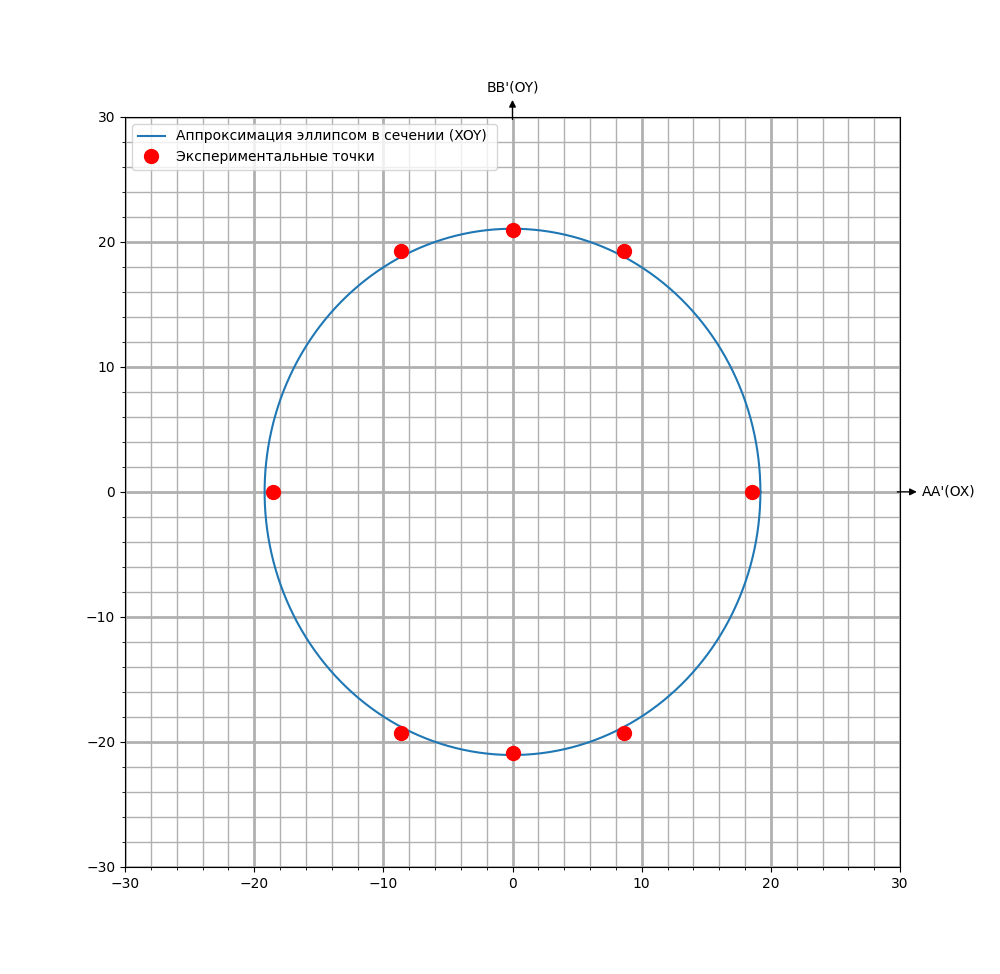
\includegraphics[width=1\textwidth]{xoy.png}
    \caption{\textit{Сечение эллипсоида инерции параллелепипеда в плоскости XOY}}
    \label{xoy}
\end{figure}

\begin{figure}[h!]
    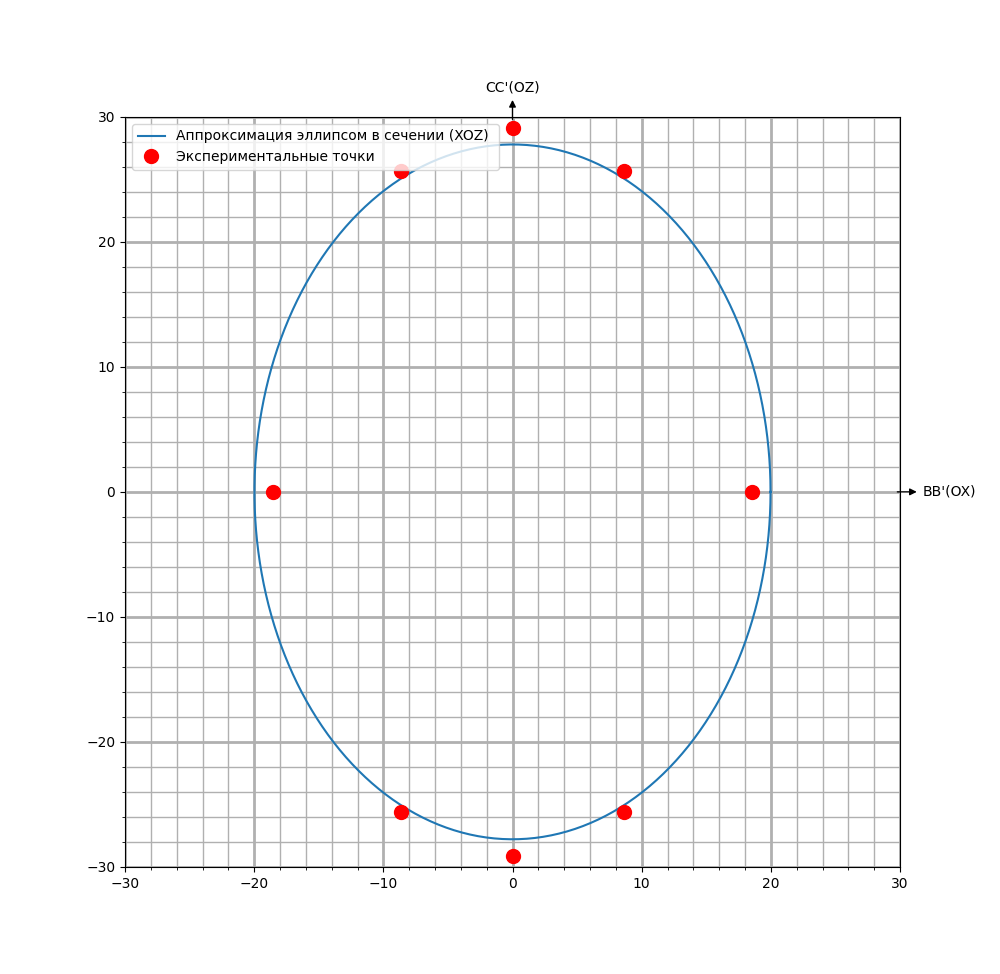
\includegraphics[width=1\textwidth]{xoz.png}
    \caption{\textit{Сечение эллипсоида инерции параллелепипеда в плоскости XOZ}}
    \label{xoz}
\end{figure}

\begin{figure}[h!]
    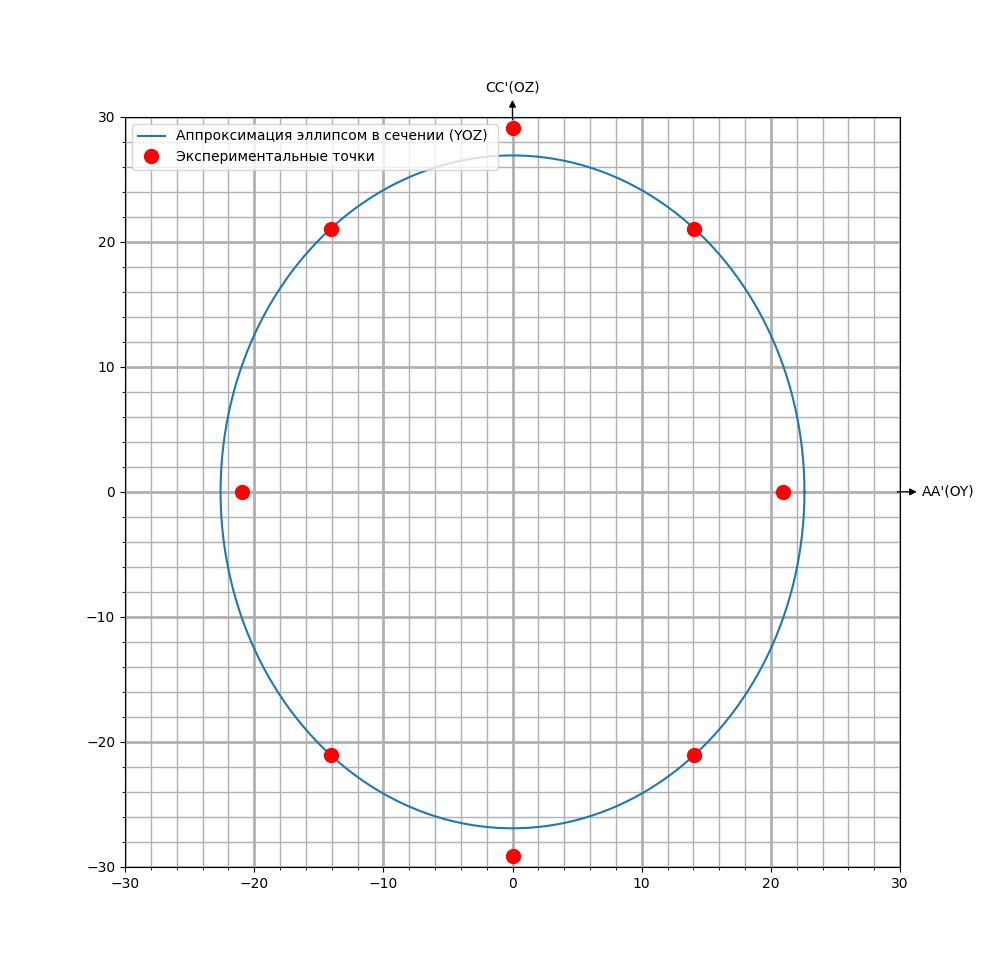
\includegraphics[width=1\textwidth]{yoz.png}
    \caption{\textit{Сечение эллипсоида инерции параллелепипеда в плоскости YOZ}}
    \label{yoz}
\end{figure}

\begin{figure}[h!]
    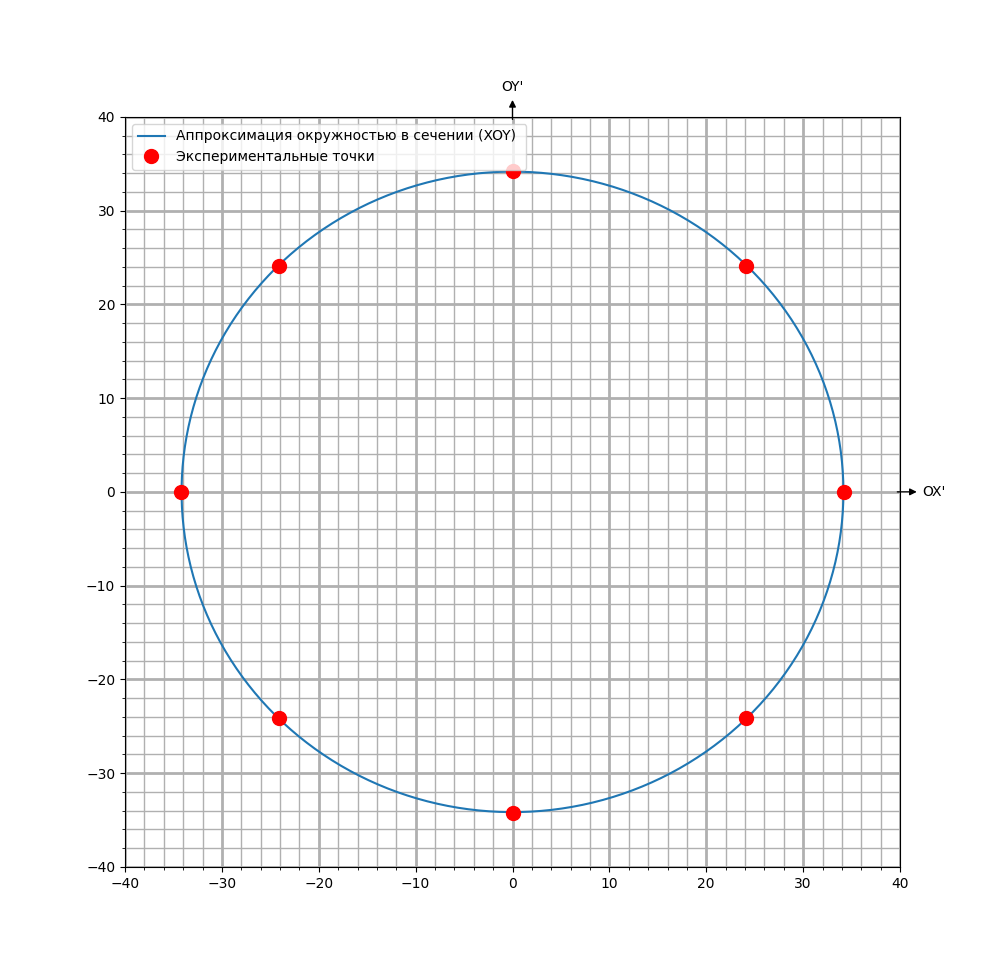
\includegraphics[width=1\textwidth]{cube-ell.png}
    \caption{\textit{Сечение эллипсоида инерции куба}}
    \label{cube-ell}
\end{figure}

\begin{figure}[h!]
    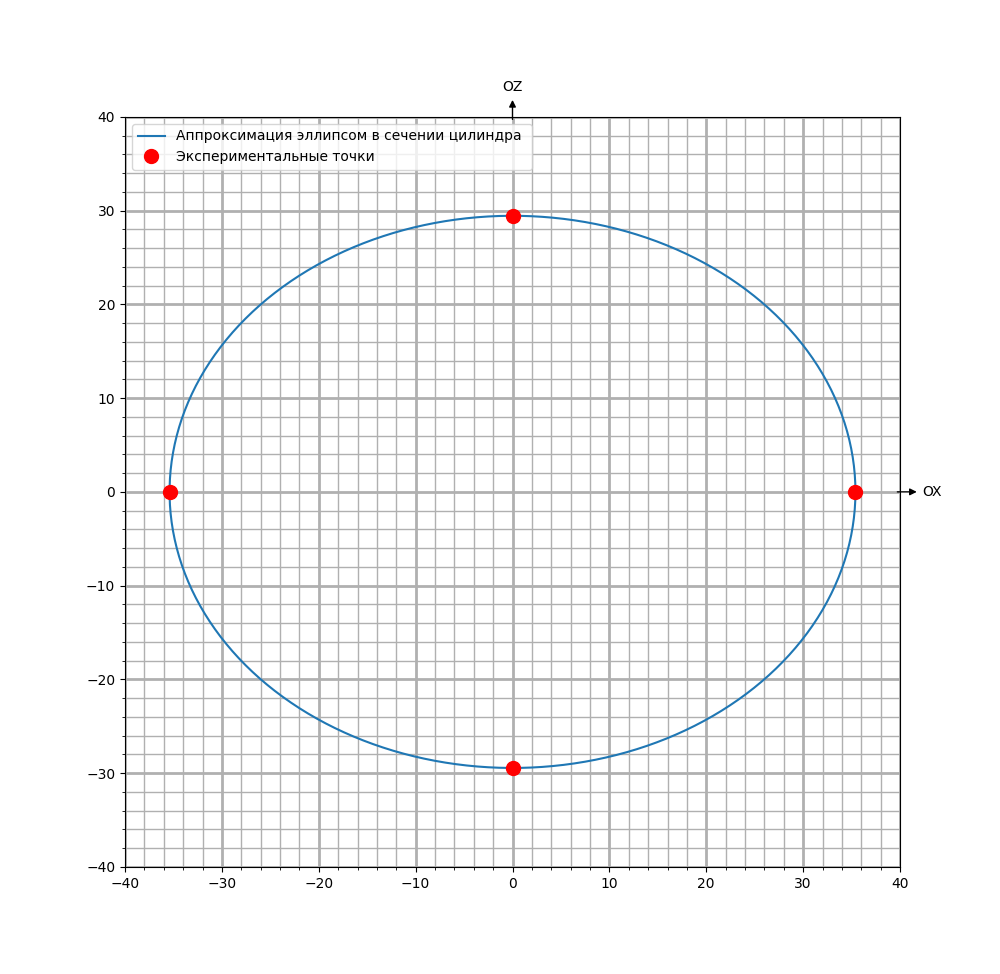
\includegraphics[width=1\textwidth]{cil.png}
    \caption{\textit{Сечение эллипсоида инерции для цилиндра}}
    \label{cil-ell}
\end{figure}

\begin{figure}[h!]
    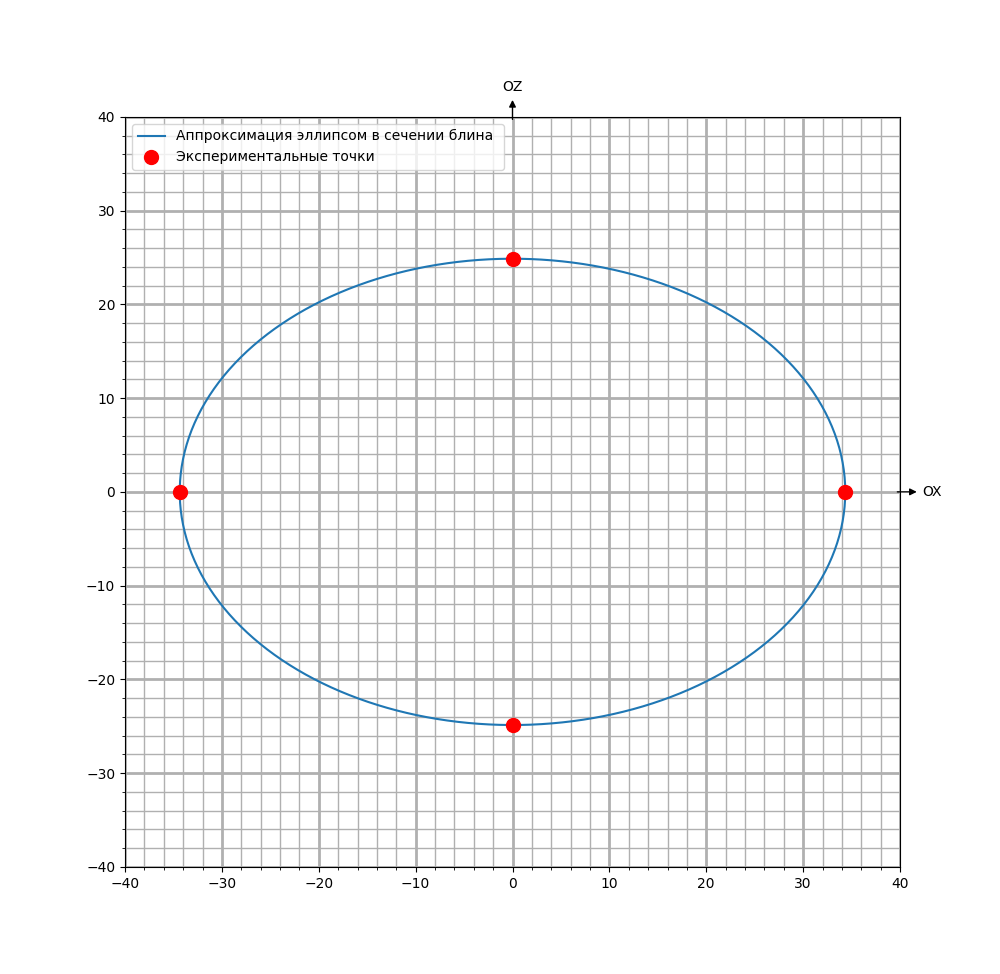
\includegraphics[width=1\textwidth]{blin.png}
    \caption{\textit{Сечение эллипсоида инерции для блина}}
    \label{blin-ell}
\end{figure}

\begin{figure}[h!]
    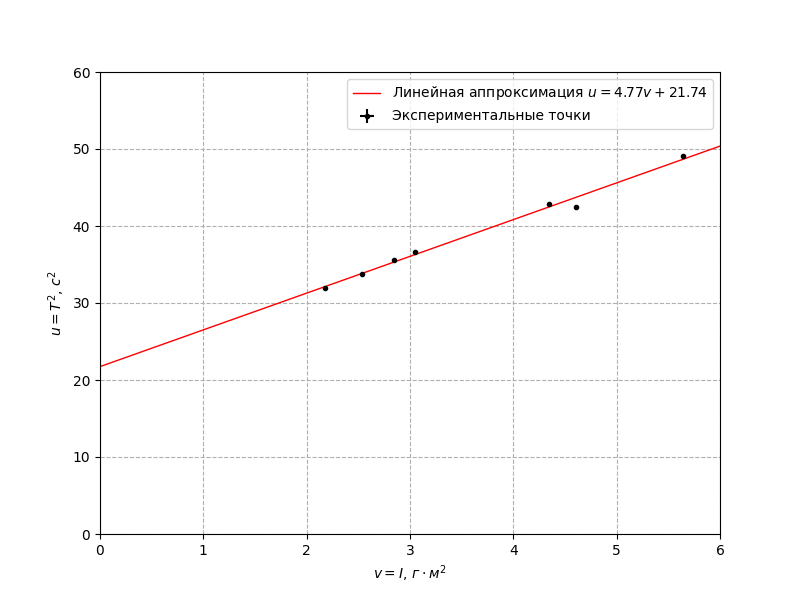
\includegraphics[width=1\textwidth]{graph.png}
    \caption{\textit{Сечение эллипсоида инерции для блина}}
    \label{T2I}
\end{figure}

\end{document}
